\begin{appendices}
\chapter{Appendix}
\label{cha:Appendix}

\section{Requirements}
\label{sec:RequirementsAppendix}

\subsection{Functional Requirements}
\label{subsec:Functional Requirements Appendix}
\begin{longtable}{|p{0.1\linewidth}|p{0.4\linewidth}|p{0.1\linewidth}|p{0.4\linewidth}|}
% Headings and Footers %
\caption{Functional requirements table.}\label{tab:functionalRequirementsAppendix}\\
\hline
\multicolumn{2}{|l|}{User Requirements} & \multicolumn{2}{l|}{System Requirements} \\
\hline
\endfirsthead

\hline
\multicolumn{2}{|l|}{User Requirements} & \multicolumn{2}{l|}{System Requirements} \\
\hline
\endhead

\hline
\endfoot

\hline
\endlastfoot

% Data %
\multirow{3}{*}{FU.1} & \multirow{3}{*}{\parbox{\linewidth}{Users can run merge simulations.}} 
 & FS.11 & The system has controls for starting merge simulations \\
 &  & FS.12 & The system can create merge simulations \\
 &  & FS.13 & The system can run merge simulations \\
\hline
\multirow{2}{*}{FU.2} & \multirow{2}{*}{\parbox{\linewidth}{User can manipulate the running speed of a simulation.}}
 & FS.21 & The system has controls changing the speed of running simulations. \\
 &  & FS.22 & Merge simulations can have their run speed changed. \\ 
\hline
\multirow{2}{*}{FU.3} & \multirow{2}{*}{\parbox{\linewidth}{User can pause simulations.}}
 & FS.31 & The system has controls to pause simulations. \\
 &  & FS.32 & Merge simulations can be paused \\ 
\hline
\multirow{2}{*}{FU.4} & \multirow{2}{*}{\parbox{\linewidth}{User can end a simulation.}}
 & FS.41 & The system has controls to end simulations. \\
 &  & FS.42 & Merge simulations can be ended. \\ 
\hline
FU.5 & User can view the activities of a simulation. & FS.51 & The system displays the current status of a simulation as it runs. \\
\hline
\multirow{9}{*}{FU.6} & \multirow{9}{*}{\parbox{\linewidth}{Users can export the results of a merge simulation.}}
 & FS.61 & The system has controls for exporting results data. \\
 &  & FS.62 & The system can produce a file containing results data from the simulation. \\
 &  & FS.63 & The results file contains the total throughput of the simulation. \\
 &  & FS.64 & The results file contains the ML throughput of the simulation. \\
 &  & FS.65 & The results file contains the TL throughput of the simulation. \\
 &  & FS.66 & The results file contains the maximum delay of the simulation. \\
 &  & FS.67 & The results file contains the average delay of the simulation. \\
 &  & FS.68 & The results file contains the ML average delay of the simulation. \\
 &  & FS.69 & The results file contains the TL average delay of the simulation. \\
 &  & FS.6a & The results file contains the maximum acceleration of the simulation. \\
 &  & FS.6b & The results file contains the maximum deceleration of the simulation. \\
 &  & FS.6c & The results file contains the delay for each vehicle in the simulation. \\
 &  & FS.6d & The results file contains the maximum acceleration for each vehicle in the simulation. \\
 &  & FS.6e & The results file contains the maximum deceleration for each vehicle in the simulation. \\ 
\hline
\multirow{3}{*}{FU.7} & \multirow{3}{*}{\parbox{\linewidth}{Users can select and run an S2S merge simulation.}}
 & FS.71 & The system can produce S2S simulations. \\
 &  & FS.72 & The system has controls allowing S2S simulations to be selected. \\
 &  & FS.73 & The system can run S2S simulations \\ 
\hline
\multirow{2}{*}{FU.8} & \multirow{2}{*}{\parbox{\linewidth}{Users can select a centralised merging scheme with S2S merge simulations.}}
 & FS.81 & The system can use an AIM-like merge management system for the merging zone in an S2S simulation. \\
 &  & FS.82 & The system has controls allowing users to select the merge scheme indicated in FS.81. \\ 
\hline
\multirow{2}{*}{FU.9} & \multirow{2}{*}{\parbox{\linewidth}{Users can select a decentralised merging scheme with S2S merge simulations.}}
 & FS.91 & The system can use an merge management scheme similar to that described in \citetitle{VanMiddlesworth2008} \citep{VanMiddlesworth2008}. \\
 &  & FS.92 & The system has controls allowing users to select the merge scheme indicated in FS.91. \\ 
\hline
FU.10 & Users can control the traffic level of an S2S simulation. & FS.101 & The system has controls for adjusting the traffic for an S2S simulation. \\ 
\hline
FU.11 & Users can control the TL speed limit of an S2S simulation. & FS.111 & The system has controls for adjusting the TL speed limit for an S2S simulation. \\ 
\hline
FU.12 & Users can control the ML speed limit of an S2S simulation. & FS.121 & The system has controls for adjusting the ML speed limit for an S2S simulation. \\ 
\hline
FU.13 & Users can control the TL lead in distance of an S2S simulation. & FS.131 & The system has controls for adjusting the TL lead in distance for an S2S simulation. \\ 
\hline
FU.14 & Users can control the ML lead in distance of an S2S simulation. & FS.141 & The system has controls for adjusting the ML lead in distance for an S2S simulation. \\ 
\hline
FU.15 & Users can control the merge angle of an S2S simulation. & FS.151 & The system has controls for adjusting the merge angle for an S2S simulation. \\ 
\hline
\multirow{2}{*}{FU.16} & \multirow{2}{*}{\parbox{\linewidth}{Users should be alerted of any collisions during a simulation.}}
 & FS.161 & The system should be able to alert the user if a collision occurs. \\
 &  & FS.162 & The simulation should detect collisions. \\ 
\end{longtable}

\subsection{Non-functional Requirements}
\label{subsec:Non-functional Requirements Appendix}
\begin{longtable}{|p{0.1\linewidth}|p{0.9\linewidth}|}
% Headings and footers %
\caption{Non-functional requirements table.}\label{tab:nonFunctionalRequirementsAppendix}\\
\hline
ID & Description \\
\hline
\endfirsthead

\hline
ID & Description \\
\hline
\endhead

\hline
\endfoot

\hline
\endlastfoot

% Data %
NS.1 & All system controls come from standard JComponents. \\
NS.2 & All controls are clearly labeled. \\
NS.3 & Simulation creation should take no longer than 3 seconds. \\
NS.4 & Simulations should be able to run faster than real-time. \\
NS.5 & Simulations should update the GUI frequently. \\
NS.6 & All data displayed to the user should be accurate. \\
NS.7 & All data in the results file should be accurate. \\
NS.8 & Created simulators should accurately represent their merge scenario with the provided modifier factors. \\
NS.9 & Code should be written to allow for easy expansion. \\
NS.10 & Code should be well documented. \\
NS.11 & The simulator should be integrated into the AIM4 simulator without negatively affecting the performance of AIM simulations. \\
NS.12 & It should be easy to add new simulator types in AIM4 alongside AIM and Merge simulations. \\
\end{longtable}

\section{S2S Map Calculations}
\label{sec:S2SMapCalculations}
To start with, we need to calculate the dimensions of the merging zone. The height of the merging zone will be the same as lane width of the target lane. The length can be calculated using the right-angled triangle in Figure \ref{fig:mergingZoneTriangle}. Using this triangle and some trigonometry we can calculate the length of the merge zone ($\text{mergingZoneLength}$ in Fig. \ref{fig:mergingZoneTriangle}) using equation \ref{hSin}.

\begin{figure}[htb]
\centering
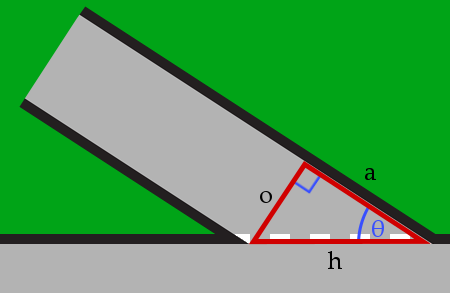
\includegraphics[width=10cm]{appendix/mergingZoneTriangle.png}
\caption{A right-angled triangle for the merging zone.}
\label{fig:mergingZoneTriangle}
\end{figure}

\begin{equation}\label{hSin}
mergeZoneLength = \frac{laneWidth}{\sin(\theta)}
\end{equation}

We also need to know whether the horizontal width of the merge lane on the map, or it's 'base width' is longer than the target lane's lead in distance, plus the merge zone length. This will determine the width of the overall map, as if the merge lane's base length is longer then the target lane will not start with co-ordinate $x=0$ as it would if the target lane determined the width of the map.

Firstly we need to calculate the X and Y adjustments at the merge lane entrance. Because the vehicles drive in the centre of the lane and the merge lead in distance is defined by the middle line of the lane we still need to calculate how far the lane extends in the x and y directions due to it's width. To do this we can use the right-angled triangles shown in Figure \ref{fig:mergeEntranceTriangles}

\begin{figure}[htb]
\centering
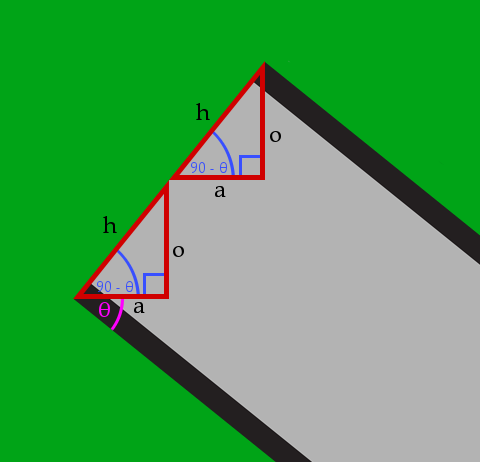
\includegraphics[width=10cm]{appendix/mergeEntranceTriangles.png}
\caption{Two right-angled triangles for the x and y adjustments.}
\label{fig:mergeEntranceTriangles}
\end{figure}

These triangles have the same dimensions and have an interior angle of 90 - $\theta$ due to the 'alternate angle' or 'z-angle' rule. Each triangle has a hypotenuse with a length equal to half the width of the lane. 

The X-adjustment for the merge entrance is the length of the adjacent side of one of the lower triangle and the Y-adjustment for the merge entrance is the length of the opposite side of the upper triangle (though both triangles do have the same dimensions). We can use equation \ref{aCos90} to calculate the X-adjustment and equation \ref{oSin90} to calculate the Y-adjustment.

\begin{equation}\label{aCos90}
\text{x-adjust} = \frac{laneWidth}{2} \cos(90 - \theta)
\end{equation}

\begin{equation}\label{oSin90}
\text{y-adjust} = \frac{laneWidth}{2} \sin(90 - \theta)
\end{equation}

To calculate the 'base width' of the merge lane we will also need to calculate the adjacent side of the triangle in Figure \ref{fig:baseWidthTriangle}. In this triangle the hypotenuse has a length equal to the merge lead in distance. Therefore, we can use equation \ref{aCos} to calculate the length of the adjacent side. After obtaining the length of this side we simply add the merge entrance X-adjustment and half the length of the merge zone to find the merge base width.

\begin{figure}[htb]
\centering
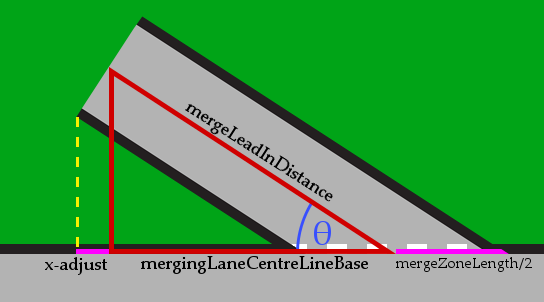
\includegraphics[width=10cm]{appendix/baseWidthTriangle.png}
\caption{A right-angled triangle for the the base width of the merge lane, with the X-adjustment and merge-zone length.}
\label{fig:baseWidthTriangle}
\end{figure}

\begin{equation}\label{aCos}
mergingLaneCentreLineBase = mergeLeadInDistance \cos(\theta)
\end{equation}

We also need to find the point at which the merging lane's centre line crosses the target lane's centre line in the merge zone. We know the Y-coordinate for this point as it will be the same as the Y-coordinate of the target lane centre line. We also know the X-coordinate of the point at which the merge lane's centre line meets the target lane. We can use these two co-ordinates to create the triangle shown in Figure \ref{fig:toCentreTriangle}. We can then use equation \ref{aTan} to find the X-adjustment from the merge zone centre to the point where the two centre lines cross.

\begin{figure}[htb]
\centering
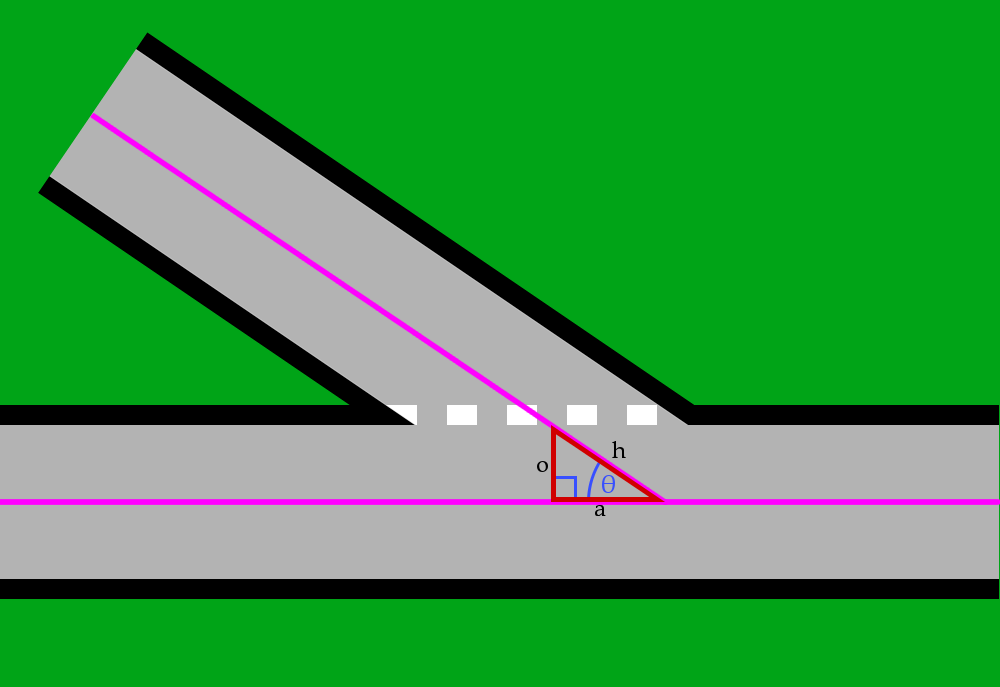
\includegraphics[width=10cm]{appendix/toCentreTriangle.png}
\caption{A right-angled triangle for lane meeting point calculations}
\label{fig:toCentreTriangle}
\end{figure}

\begin{equation}\label{aTan}
toCentreDistance = frac{laneWidth}{2 \tan(\theta)}
\end{equation}

\section{Generalising the Codebase}
\label{sec:Generalising the Codebase Appendix}
All class diagrams were created using the `IntelliJ IDEA 15.0.3' internal diagram tool. Figure \ref{fig:classDiagramKey} provides a key for understanding these diagrams.

\begin{figure}[htb]
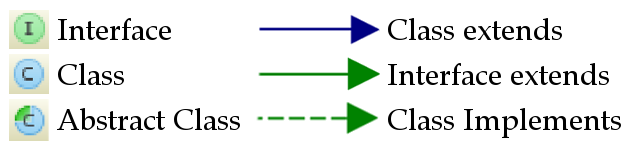
\includegraphics[width=\textwidth]{classDiagrams/classDiagramKey.png}
\caption{Key for the class diagrams in this report.}
\label{fig:classDiagramKey}
\end{figure}

\subsection{aim4.driver}
\label{subsec:aim4.driver}
\emph{aim4.driver} controls how a vehicle behaves on the map. In the original simulator the drivers were built to deal with 4-way intersections, with general functionality tied into the same class. You can see how this was done in Figure \ref{fig:driverBefore}.

\begin{figure}[htb]
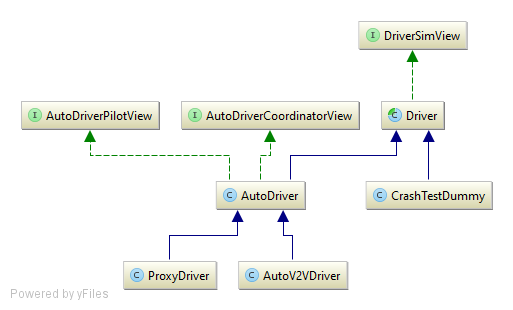
\includegraphics[width=\textwidth]{classDiagrams/driverBefore.png}
\caption{The original class structure for \emph{Driver}.}
\label{fig:driverBefore}
\end{figure}

The first major change was renaming \emph{DriverSimView}, \emph{AutoDriverPilotView}, and \emph{AutoDriverCoordinatorView} to end in \emph{Model} instead of \emph{View}. These interfaces are used to limit the methods that other classes can access in Driver and AutoDriver, thus changing their 'view' of that class. We felt that \emph{View} could cause confusion with the GUI elements of the simulator; we instead chose to refer to these interfaces as \emph{Models}, because the accessors are effectively given a model of Driver and AutoDriver (beyond which they care very little) that they can use to access methods.

The next change was separating out all of the AIM specific code into its own classes and interfaces. You can see how this was done in Figure \ref{fig:driverAfter} with \emph{AIMDriverSimModel} and \emph{AIMDriver}. The merge specific code found in \emph{MergeDriverSimModel}, \emph{MergeDriver} and \emph{MergeAutoDriver} is structured in a very similar manner to its AIM counterpart, taking advantage of the generalised code.

\begin{sidewaysfigure}[p]
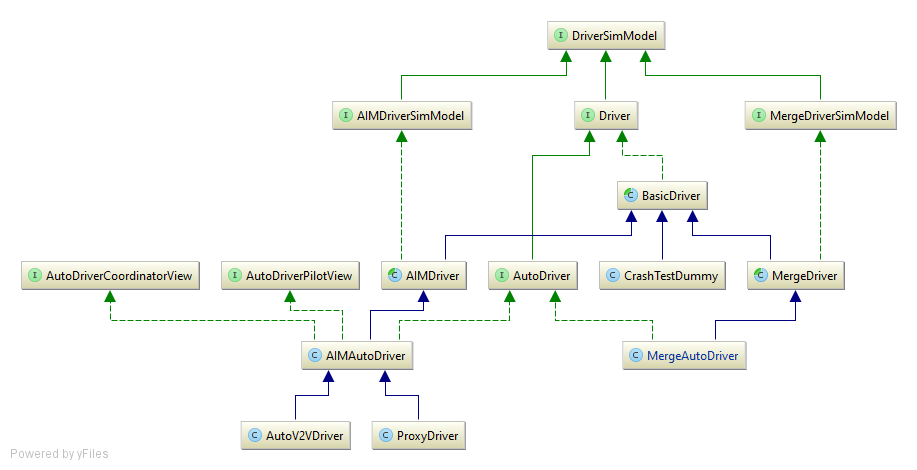
\includegraphics[width=\textwidth]{classDiagrams/driverAfter.png}
\caption{The new class structure for \emph{Driver}.}
\label{fig:driverAfter}
\end{sidewaysfigure}

As a consequence of breaking out the code like this, a number of additional changes had to be made. Driver was changed into an interface and a new class \emph{BasicDriver}. \emph{Driver} is simply used as an interface for accessing Drivers in non-simulation contexts (such as \emph{BasicVehicle}). \emph{BasicDriver} contains the generalised functionality all \emph{Driver} objects should need, with AIM specific activities moved to \emph{AIMDriver}. Extending from \emph{Driver} is the \emph{AutoDriver} interface, which adds no new methods but is instead used to categorise autonomous drivers. \emph{AIMAutoDriver} contains almost exactly the same code as the original \emph{AutoDriver} class.

\FloatBarrier
\subsection{aim4.gui}
\label{subsec:aim4.gui}
\emph{aim4.gui} controls the GUI for the simulator. We had to adjust this to allow for non-AIM simulations to be run. We chose to use tabs to allow users to switch between simulators (these are greyed out when a simulation is running). To make adding new tabs and simulation screens easier we had to refactor \emph{Viewer} into smaller, separate components.

In the original simulator \emph{Viewer} displays the simulator set-up controls, \emph{SimSetupPanel}, and the simulation viewer \emph{Canvas} inside \emph{mainPanel}. \emph{mainPanel} is a \emph{JPanel} with a \emph{CardLayout} allowing the panel to switch between displaying the set-up controls and the viewer. In the new simulator we replaced \emph{mainPanel} with \emph{tabbedPane}, a \emph{JTabbedPane} object that allows users to switch between the different simulators using tabs. Each tab displays a \emph{SimViewer}, which behaves in a similar way to \emph{mainPanel} allowing users to switch between the set-up screen and the simulation screen using \emph{CardLayout}. Each simulator will have their own SimViewer type, as shown in Figure \ref{fig:simViewer}.

\begin{figure}[htb]
\centering
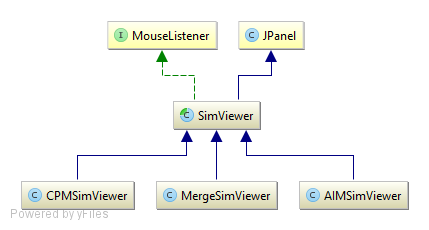
\includegraphics[width=8cm]{classDiagrams/simViewer.png}
\caption{The class diagram for \emph{SimViewer}.}
\label{fig:simViewer}
\end{figure}

We didn't want to force new simulators to use a full representation of vehicles on screen, as \emph{Canvas} does. To avoid this we created a new interface \emph{SimScreen} which \emph{SimViewer} uses to describe it's viewer card. Any class implementing \emph{SimScreen} can be used as the viewer for a simulation. Figure \ref{fig:simScreen} shows how \emph{MergeStatScreen} and \emph{Canvas} using \emph{SimScreen}.

\begin{figure}[htb]
\centering
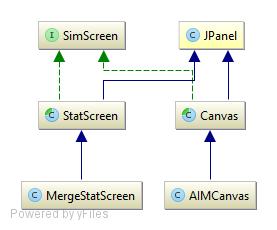
\includegraphics[width=8cm]{classDiagrams/simScreen.png}
\caption{The class diagram for \emph{SimScreen}.}
\label{fig:simScreen}
\end{figure}

We also generalised the \emph{SimSetupPanel} class to allow \emph{SimViewer} to display non-AIM set-up controls. Figure \ref{fig:simSetupPanel} shows the new class structure for \emph{SimSetupPanel}.

\begin{figure}[htb]
\centering
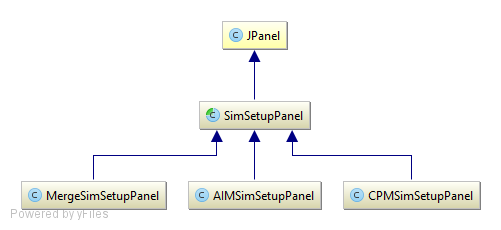
\includegraphics[width=8cm]{classDiagrams/simSetupPanel.png}
\caption{The class diagram for \emph{SimSetupPanel}.}
\label{fig:simSetupPanel}
\end{figure}

We also made a small adjustment to the behaviour of the reset option in the menu. Now the simulator must be paused in order for the reset button to be active. We did this because resetting the simulator without pausing was creating \emph{NullPointerException}s.

\FloatBarrier
\subsection{aim4.map}
\label{subsec:aim4.map}
\emph{aim4.map} is used to describe the environment vehicles are required to navigate. They also spawn vehicles that then drive through the map. Figures \ref{fig:mapBefore} and \ref{fig:mapAfter} show the original and new class structure for \emph{aim4.map}.

\begin{figure}[htb]
\centering
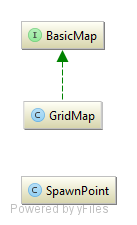
\includegraphics[height=6cm]{classDiagrams/mapBefore.png}
\caption{The original class structure for \emph{BasicMap} and \emph{SpawnPoint}.}
\label{fig:mapBefore}
\end{figure}

\begin{figure}[htb]
\centering
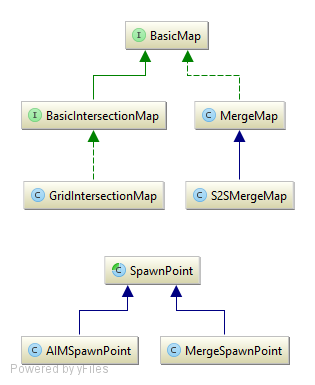
\includegraphics[width=8cm]{classDiagrams/mapAfter.png}
\caption{The new class structure for \emph{BasicMap} and \emph{SpawnPoint}.}
\label{fig:mapAfter}
\end{figure}

The changes made to \emph{aim4.map} were relatively straight-forward. The AIM specific features in \emph{BasicMap} were extracted out in \emph{BasicIntersectionMap} and \emph{GridMap} was renamed to \emph{GridIntersectionMap} and now inherits from the new interface. This allows for new map types, such as \emph{MergeMap} to implement a map type without AIM features.

\emph{SpawnPoint} was also broken out into general and AIM specific features. This had to be done because \emph{SpawnPoint} used to create \emph{SpawnSpec} objects with \emph{destination} fields. \emph{destination} is an AIM specific field relating to the intersection exit a vehicle plans to reach. By extracting this out new map types can spawn vehicles with \emph{SpawnSpec} instances specific to their map type.

\FloatBarrier
\subsection{aim4.sim}
\label{subsec:aim4.sim}
\emph{aim4.sim} contains the code responsible for constructing and running simulations. The original code was very focussed on AIM simulations and so we had to break the interfaces to allow for different types of simulators. 

\emph{Simulator} is an interface that new simulators need to implement. We decided to extract out some of the AIM specific features into \emph{AIMSimulator}. We also added an override to \emph{getMap()}, forcing AIM simulators to use \emph{BasicIntersectionMap} maps. The class structure changes can be seen in Figures \ref{fig:simulatorBefore} and \ref{fig:simulatorAfter}.

\begin{figure}[htb]
\centering
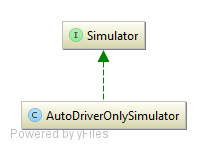
\includegraphics[width=8cm]{classDiagrams/simulatorBefore.png}
\caption{The original class structure for \emph{Simulator}.}
\label{fig:simulatorBefore}
\end{figure}

\begin{figure}[htb]
\centering
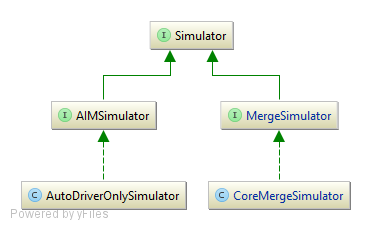
\includegraphics[width=12cm]{classDiagrams/simulatorAfter.png}
\caption{The new class structure for \emph{Simulator}.}
\label{fig:simulatorAfter}
\end{figure}

\emph{SimSetup} was also modified to separate AIM specific set-up options and simulator creation code from other simulators.

\FloatBarrier
\subsection{aim4.vehicle}
\label{subsec:aim4.vehicle}
\emph{aim4.vehicle} controls the different vehicles used during simulations. Vehicles are used by both \emph{Driver} and \emph{Simulator} instances. To allow them to do that the original simulator code used \emph{View} interfaces similar to those in \ref{subsec:aim4.driver}. Figure \ref{fig:vehicleBefore} shows how these interfaces link together. Extracting AIM behaviour was quite difficult because of how interconnected these interfaces were. The solution we came up with was to create AIM specific interfaces and link them together in a similar manner, inheriting from the generic ones if possible. Figure \ref{fig:vehicleAfter} shows how the new structure links together.

\begin{figure}[htb]
\centering
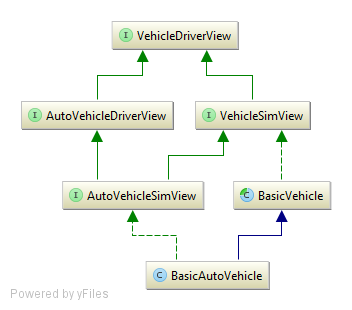
\includegraphics[width=10cm]{classDiagrams/vehicleBefore.png}
\caption{The original class structure for \emph{aim4.vehicle}.}
\label{fig:vehicleBefore}
\end{figure}

\begin{sidewaysfigure}[p]
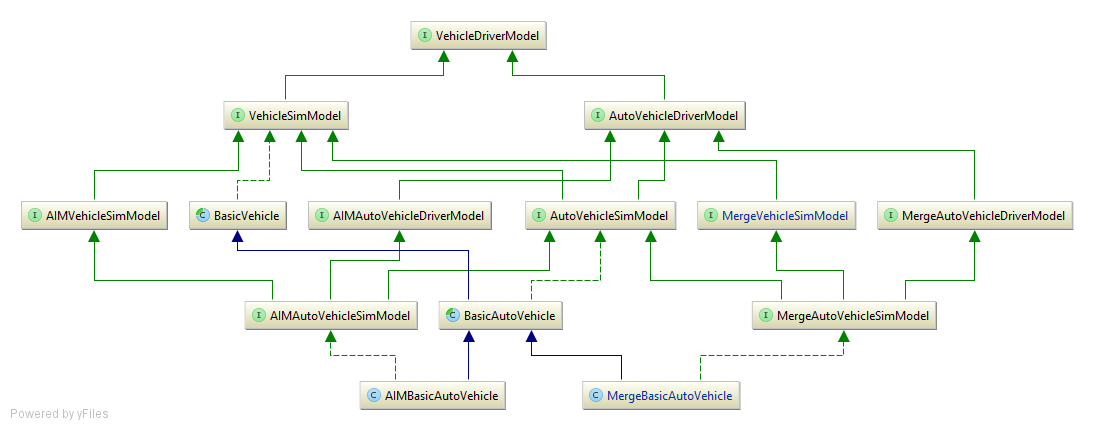
\includegraphics[width=\textwidth]{classDiagrams/vehicleAfter.png}
\caption{The new class structure for \emph{aim4.vehicle}.}
\label{fig:vehicleAfter}
\end{sidewaysfigure}

The first change made to \emph{aim4.vehicle} was to rename all of the files ending in \emph{View} to end in \emph{Model} instead. This matches the changes made to \emph{aim4.driver}.

\emph{AIMVehicleSimModel} and \emph{AIMAutoVehicleDriverModel} are at the top of the AIM interface tree. They both extend their generic counterparts. \emph{AIMAutoVehicleSimModel} extends these two interfaces along with \emph{AutoVehicleSimModel}. This matches up to the original inheritance structure. Any future vehicles will need to create their own version of these interfaces, as seen in \emph{MergeVehicleSimModel}, \emph{MergeAutoVehicleDriverModel} and \emph{MergeAutoVehicleSimModel}. 

In terms of classes we made \emph{BasicAutoVehicle} abstract and extracted out AIM specific behaviour to \emph{AIMBasicAutoVehicle}. \emph{BasicAutoVehicle} had to be abstract because we wanted to force \emph{getDriver()} to be overridden in subclasses to retrieve the simulator specific \emph{AutoDriver} for that vehicle (for example \emph{AIMAutoDriver} in AIM simulators). 

\FloatBarrier
\section{Lead in Distance Analysis}
\label{sec:Lead in Distance Analysis}
The lead in distance adjustments affect how long vehicles have to organise and communicate with QMM. Different lead in distance pairs were tested. The traffic rate was set to 1000\si{vhl}, the merge angle was set to 45\degree, and the speed limit was set to 20$\si{ms^{-1}}$ (44.7\si{mph} or 72\si{kph}).

Due to the 150\si{m} distance limit on requests, lead ins at 100\si{m} were worse for the lane with the 100\si{m} lead in. The only exceptions were when both lanes had lead in distances of 100\si{m}.

If one lane has a 100\si{m} lead, then the other lane also suffers a performance hit. This affect is most noticeable when the target lane has the 100\si{m} lead, but this effect is also seen with the merge lane. 

Beyond 150\si{m} the lead in distance had very little effect on the performance of the system. Throughput remained relatively constant throughout. Appendix \ref{fig:meanDelayLeadIn} shows how the mean delay relates to the lead in distance.

\begin{figure}[p]
\centerline{
	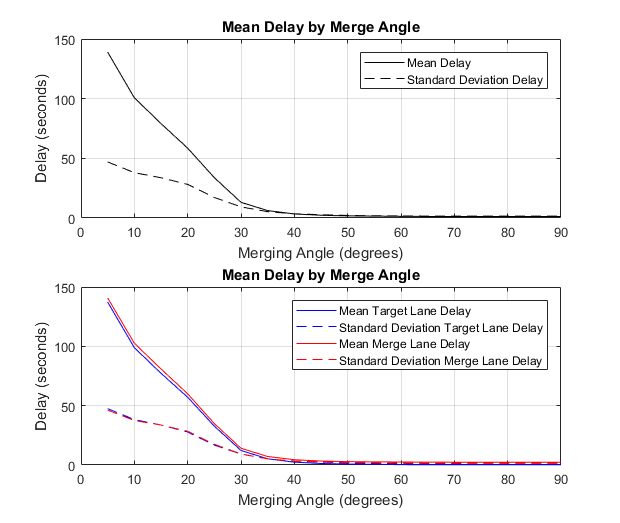
\includegraphics[height=\textheight]{plots/leadIn/meanDelay.png}
}
\caption{Bar chart showing mean delay by lead in distance}
\label{fig:meanDelayLeadIn}
\end{figure}
\end{appendices}